\chapter{Probabilistic Vector Machines}\label{Pc}
In this chapter, the \ac{PCVM} and previous work is described.
It is developed by Huanhuan Chen et al. in the corresponding article \cite{Chen.2009}. 
However, first, we look at some disadvantages of the \ac{SVM}.
The idea of the \acs{RVM} are mainly motivated to improve and solve the \acs{SVM}.\cite[p. 1-2]{Tipping.2001}
Moreover, finally, the \acs{PCVM} is developed to cure some conception assumptions, which are leading in the opinion of Chen et al. to unstable results.
Regarding to Chen et al. sees the \acs{PCVM} as improved version of the \acs{RVM}.\cite{Chen.2009}\newline
\section{Disadvantages of Support Vector Machines}\label{PcSecIdea}
At first the \acs{SVM}, which is described as baseline classifier in section \ref{EmSubSecSVM}, provides a optimal solution through the convex optimization problem \cite[p. 325]{Bishop.2009}, but suffers from a few disadvantages.\newline
The \acs{SVM} is non probabilistic.
The problem is that the hard binary decisions which are made of the \acs{SVM} are not made to catch the uncertainty for predictions.
Furthermore, the probabilistic predictions are considered as crucial when posterior probabilities of a class assignment are adapted to varying class priors and asymmetric misclassification costs.\cite[p. 239-240]{Tipping.2001}\\
To solve this problem, there are some post processing methods developed to match the binary import to a probabilistic output.
However, this is considered as unreliable by \cite[p. 239-240]{Tipping.2001}. 
This uncertainty can be interpreted as Bayesian probability.\cite[p. 21]{Bishop.2009}\newline 
Second, the number of support vectors needed to create the margin of the decision boundary grows linearly with the size of the training set.
With that, the computational complexity and model complexity grows and does not lead to sparse models or fast computing.
As a consequence, some post-processing is suggested to reduce the complexity of the model.\cite{Chen.2009}\\
An example would be to find a set of 'reduced' vectors with $N_\mathcal{Z}$ entries, which are approximate the original set of support vectors $N_S$.
Note that these reduced vectors are no training samples and are not necessarily lying on the margin.
The goal is then to find the smallest $N_\mathcal{Z}$ with $N_\mathcal{Z} \ll N_S$ for that the loss in the generalisation performance is acceptable.
However, this approach is computational very expensive.\cite{Burges.1997}\\
Therefore the wanted reduction of computational complexity is maybe not yet achieved.\newline
Furthermore, the \ac{SVM} has several parameters, that needs to be tuned by cross-validation.
For example the $C$ parameter, explained in section \ref{EmSubSecSVM}, or the parameters for the kernel function for example the width of the Gaussian kernel, section \ref{EmSubSecKernel}.
Cross-validation is done by a grid search in a certain range.
For example evaluate the performance of the \ac{SVM} for $C={1,2,5,10,...,100,200}$ and select the parameter according to the best performance.\cite{Chen.2009}\newline
Finally, when it comes to the interpretation of the results, the \ac{SVM} provides a good interpretation of how the margin and the decision boundary is created.
However, the points which are considered as support vectors and therefore selected in the model, are not representing the actual data very well, because they are the closest points from one class to the other class.\cite[p. 326]{Bishop.2009}\newline
Here a key feature from the \ac{RVM} takes place. It creates a sparser model, in comparison with the \ac{SVM}, and provides a probabilistic estimate of the classes, where the relevance vectors are representing the data.\cite[p. 335-356]{Bishop.2009}\newline
This effect can be seen in figure \ref{FigRVMProbEst}.
One the right, the circled points are the relevance vectors of the model and on the right the posterior probability for the classes as colour gradient respectively.
\begin{figure}
	\centering
	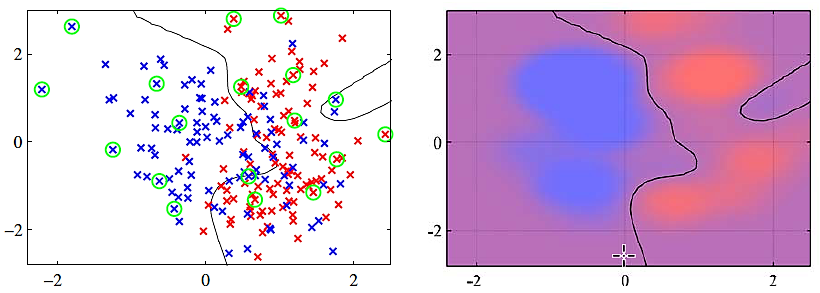
\includegraphics[width=.8\linewidth]{figures/RVMProbEst.png}
	\caption[Probabilitc Estimate of the RVM]{The probabilistic estimate of the \acs{RVM} on a synthetic dataset. The green circled points are relevance vectors.\cite[p. 356]{Bishop.2009}}
	\label{FigRVMProbEst}
\end{figure}

\section{Relevance Vector Machine}\label{PcSecRVM}
The \ac{RVM} is introduced by Tipping in the already noted work \cite{Tipping.2001}.
The key idea behind it is to create a classifier with a similar functional form to the \ac{SVM} with a probabilistic background. 
It uses a general Bayesian framework.\newline
The \acs{RVM} uses relevance vectors instead of support vectors.
It is found that for many weights the posterior distribution is sharply peaked around zero.
That means the probability for a certain weight for the training point is highest nearly the weight zero.
The training vectors with the corresponding remaining non-zero weights are called relevance vectors.
The weights representing the importance of a relevance vector.\cite[p. 213]{Tipping.2001}
Note that although in this thesis the same letter is used for the parameter $\mathbf{w}$, there is an important difference between them.
The \acs{SVM} defines with this parameter the hyperplane and the probabilistic vector machines are more prototypical vectors, which are representing the corresponding class in a probabilistic manner shown in figure \ref{FigRVMProbEst}.\cite[p. 222]{Tipping.2001}\newline
Another advantage of the \acs{RVM} against the \acs{SVM} is , that the kernel function for a \acs{SVM} has to satisfy Mercer's conditions.
The \ac{RVM} kernel does not have this constraint.\cite[p. 213]{Tipping.2001}\newline
Without going deeper in this, a kernel which satisfies the Mercer's conditions is positive semi-definite.\cite{Graepel.2002}
The complexity of the algorithm is $\mathcal{O}(M^3)$ with $M$ as number of basis functions and is also similar to the \ac{SVM}.\cite[p. 236-237]{Tipping.2001}\newline
The \ac{RVM} makes predictions for a new point $\mathbf{x}$ with equation \ref{EqRVMPred}.\cite[p. 211]{Tipping.2001}
\begin{equation}\label{EqRVMPred}
	\mathbf{t} = y(\mathbf{x};\mathbf{w}) = \sum_{i=1}^{N}\phi_i(\mathbf{x})w_i + w_0 = \boldsymbol{\Phi}(\mathbf{x})\mathbf{w} + w_0
\end{equation}
With the bias $w_0$ and basis function $\boldsymbol{\Phi}(\mathbf{x}) = (\phi(\mathbf{x_1}),\dots,\phi(\mathbf{x_n}))$.
The weight parameter has the form $\mathbf{w} = (w_1,\dots,w_N)^T$ and $\mathbf{T}={t_1,\dots,t_N}$ as function value.\\
In \eqref{EqRVMPred}, the bias is used to move the model out of the origin.
The corresponding label of a data point is the sign of the function value $\mathbf{t}$.
In general $t$ is the regression value. \cite[p. 662]{Theodoridis.2015} \newline
As a consequence, to being able to solve \eqref{EqRVMPred}, the weight $\mathbf{w}$ with size $N$ and $w_0$ has to be determined.
For the classification, the \acs{RVM} uses the Bayesian theorem in \eqref{EqBayesInfeRVM} do determine the weights $\mathbf{w}$. 
\begin{equation}\label{EqBayesInfeRVM}
	p( \mathbf{w}\vert \mathbf{t} ) \propto P(\mathbf{t}\vert \mathbf{w}) p(\mathbf{w} \vert \boldsymbol{\alpha})
\end{equation}
Note that the regression is varying from the classification solution.
The \ac{RVM} for classification gives the probability of a label for a point $\mathbf{x}$ by applying a logistic sigmoid function, with $y=y(\mathbf{x})$, which gives the probabilistic output:
\begin{equation}\label{EqLogSig}
	\sigma=1/(1+e^{-y}) 
\end{equation}
Furthermore, the logistic sigmoid function is combined with the Bernoulli distribution of $P(t\vert \mathbf{x})$ for the likelihood:
\begin{equation}\label{EqRVMLikelihood}
	P(\mathbf{t}\vert\mathbf{w})=\prod_{n=1}^{N}\sigma\{y(\mathbf{x}_n;\mathbf{w})\}^{t_n}[1-\sigma\{y(\mathbf{x}_n;\mathbf{w})\}]^{1-t_n}
\end{equation}
The Bernoulli distribution can be obtained from \cite[p. 685]{Bishop.2009} .
Additionally, the prior $p(\mathbf{w} \vert \boldsymbol{\alpha})$ is obtained by a zero-mean Gaussian:
\begin{equation}\label{EqRVMPrior}
	p(\mathbf{w} \vert \boldsymbol{\alpha}) = \prod_{i=0}^{N}\mathcal{N}(w_i\vert 0,a_i^{-1})
\end{equation}
With the inverse hyperparameter vector $\boldsymbol{\alpha}$ of size $N+1$ as the precision of the Gaussian.
At this point the parameter $w_0$ from \eqref{EqRVMPred} is determined.
The parameter $\boldsymbol{\alpha}$ itself is Gamma distributed.\cite[p. 214-215, 218-219]{Tipping.2001}\newline
An idea of a Gamma distribution and the Bernoulli distribution can be obtained from \cite[p.686-688]{Bishop.2009}.\newline
Because the integral of the Bayesian inference is intractable the following procedure is used to determine the parameters:
The algorithm is trained with the resulting Hessian Matrix from likelihood and prior of \ref{EqBayesInfeRVM}.
The most probable weights $\mathbf{w}_{MP}$ and the corresponding covariance matrix $\boldsymbol{\Sigma}$ are obtained from the mode of the posterior and the Hessian:
\begin{equation}
	\begin{split}
		\boldsymbol{\Sigma} = (\boldsymbol{\Phi}^T\mathbf{B}\boldsymbol{\Phi} + \mathbf{A})^{-1}\\
		w_{MP}=\boldsymbol{\Sigma}\Phi^T\mathbf{B}\mathbf{t} 
	\end{split}
\end{equation}
Where $\mathbf{A} = diag(\alpha_1,\dots,\alpha_N)$ and $\mathbf{B} = diag(\beta_1,\dots,\beta_N)$ with $\beta_n =\sigma\{y(\mathbf{x}_n)\}[1-\sigma\{y(\mathbf{x}_n)\}]$.
After the update of $\mathbf{w}_{MP}$ and $\boldsymbol{\Sigma}$ the hyperparameters are updated.
This is repeated until $\boldsymbol{\alpha}$ satisfies a stable convergence criteria.\cite[p. 219]{Tipping.2001}\newline
Although Tipping solved the problems of the \ac{SVM} with the \ac{RVM}, Chen et al. proposed that there are some concept problems left.\cite{Chen.2009}
These are discussed in the following sections, especially section \ref{PcSecWeights}.
\section{Probabilistic Classification Vector Machine}\label{PcSecAdvan}
In general, the \acf{PCVM} should provide a more stable solution, sparser model and better performance in comparison with the \acs{SVM} and \acs{RVM}.\cite{Chen.2009}\\
The \ac{PCVM} uses a latent variable model because of the assumption that the data is incomplete or latent.
Because of this and because the integral of the Bayesian Inference is in this case intractable, it uses an \ac{EM} algorithm, as it is a general solution to get a \ac{MAP} estimation of parameters based on latent variables.
Furthermore, the \acs{EM} algorithm optimises the parameters within, and therefore the \ac{PCVM} does not need cross-validation because the free model parameter is optimised within the algorithm.\cite{Chen.2009}\newline
An Attribute of the \acs{EM} algorithm is that it is likely to be trapped in local maxima and therefore finds no global solution.\cite{YiWang.2006}
Unlike to the \acs{SVM} which always can determine the global maxima, see section \ref{EmSubSecSVM}.\newline

\subsection{Model Specification}\label{PcSecCM}
The \acs{PCVM} is made for binary classification\cite{Chen.2009}, unlike the \acs{RVM}, which has a specification for multi class.\cite[p. 220]{Tipping.2001} But the ideas behind the two concepts are similar as we will see in the following.\\
In general, it makes predictions for a given test point $\mathbf{x}$ with the already known prediction function from \eqref{EqRVMPred} and \eqref{EqSVMPred}.\cite{Chen.2009}
As well as the \acs{RVM} in section \ref{PcSecRVM}, the \acs{PCVM} uses a link function to match the linear to a probabilistic output.
In the PCVM it is done with the probit link function defined in \ref{EqPcvmProbit}:\cite{Chen.2014}
\begin{equation}\label{EqPcvmProbit}
	\Psi(\mathbf{x}) = \int_{-\infty}^{x}N(t\vert 0,1)dt
\end{equation}
Where $\Psi$ is the Gaussian \ac{CDF}, with mean zero and variance one.\\
With a \ac{CDF} the probability for a new point x of a steady random variable X can be determined.
It is the integral of the density function and gives the probability $P(X \le x)$, which means the probability that X takes a value equals or less of x.\cite[p. 270]{Teschl.2014}\\
Therefore the probabilistic model after integrating the probit link function becomes:
\begin{equation}
	l(\mathbf{x};\mathbf{w};b) = \Psi\bigg(\sum_{i=1}^{N}w_i\phi_{i,\theta}(\mathbf{x}+b \bigg) = \Psi(\boldsymbol{\Phi}_\theta(\mathbf{x})\mathbf{w}+b)
\end{equation}
Where $\boldsymbol{\Phi(\mathbf{x})}_\theta=(\Phi_{1,\theta}(\mathbf{x}),\dots,\Phi_{N,\theta}(\mathbf{x}))$ and $\mathbf{w} = (w_1,\dots,w_N)^T$is the basis function vector with $N$ training data points.
$\theta$ is the parameter of the basis function. As the \ac{PCVM} uses the Gaussian kernel as basis function therefore the parameter $\theta$ is referred as the width of the kernel.\cite{Chen.2009}
The Gaussian kernel is described in the section \ref{EmSubSecKernel}.
\subsection{Prior over Weights}\label{PcSecWeights}
The three algorithms \acs{SVM}, \acs{RVM} and \acs{PCVM} are determining the weight parameter differently.\\
It is important for a stable solution that the sign of the weight $w_i$ of a data point $\mathbf{x}_i$ is equal to the corresponding classes $y_i \in\{-1,+1\}$.\cite{Chen.2009}\\
The \ac{SVM} ensures this by defining the weight vectors as $\mathbf{w} = \{v_1y_1,\dots,v_ny_n\}$, where $v_i$ are non negative Lagrange multipliers.
Therefore the same sign is guaranteed.\cite{Chen.2009}
But consider, that some of the data points which are not support vectors have $v_i=0$.\cite[p. 330]{Bishop.2009} \\
The \ac{RVM} estimates the weights according to equation \eqref{EqBayesInfeRVM}.
The likelihood is always positive because exponential function $e$ is always positive \cite[p. 355]{Hartmann.2015} and hence the logistic sigmoid link function is it.
Therefore the sign depends on the prior, which uses the zero-mean Gaussian over all weights and hence providing some problems.\\
It can happen that training errors occur with the use of the zero-mean Gaussian because the weight of a positive relevance vector can get a negative weight assigned and vice versa.
This may lead to an unstable result corresponding to nonreliable vectors.
As a consequence, the \acs{RVM} is more likely to overfit the noise in comparison with the \acs{SVM} and \acs{PCVM}, with the same selection of parameters.\cite{Chen.2009}\\
At this point the improvements of the \acs{PCVM} take place. 
Instead of the zero-mean Gaussian prior, it uses the zero-mean truncated Gaussian as prior. \cite{Chen.2009}
\begin{equation}\label{EqPcvmNtPrior}
	p(\mathbf{w} \vert \boldsymbol{\alpha}) = \sum_{i=1}^{N}p(w_i \vert \alpha_i) = \sum_{i=1}^{N}N_t(w_i \vert 0,\alpha_i^{-1})
\end{equation}
Here $N_t$ is the truncated Gaussian function with $\alpha$ as inverse variance.\\
With that, the relevance vector is always getting the proper signed weight attached.
Because for $y_i=+1$ the prior is selected from the right-truncated non-negative Gaussian and for $y_i=-1$ it is the left-truncated non-positive Gaussian.\cite{Chen.2009}\\
Now to avoid errors corresponding to noise or unreliable points the above is formulated in \eqref{EqPcvmWSel}.\cite{Chen.2009}
\begin{equation}\label{EqPcvmWSel}
	p(w_i \vert \alpha_i) =
	\begin{dcases*}
		2N(w_i \vert 0,\alpha_i^{-1} ),\>\>\>\>  if y_i w_i \ge 0\\
		0				,\>\>\>\>\>\>\>\>\>\>\>\>\>\>\>\>\>\>\>\>\>\>\>\>\>\>\>\> if y_i w_i<0
	\end{dcases*}
\end{equation}
With that, the \acs{PCVM} assigns for an unreliable point a zero weight, and therefore there it is no longer considers as relevance vector for the model.
The truncated Gaussian priors are illustrated in figure \ref{FigTruncGaus}.\newline
The bias $b$ which is referred as $w_0$ in \eqref{EqRVMPrior} is still determined with the zero-mean Gaussian:\cite{Chen.2009}
\begin{equation}\label{EqPcvmBPrior}
p(b \vert \beta) = N(b \vert 0, \beta^{-1})
\end{equation}
\begin{figure}
	\centering
	\floatbox[{\capbeside\thisfloatsetup{capbesideposition={right,top},capbesidewidth=6cm}}]{figure}[\FBwidth]
	{\caption[Truncated Gaussian Priors over Weights]{The truncated Gaussian priors over weights.On the left side the non positive left-truncated one in case of a negative class labels. On the right side the non negative right-runcated one for the positive class.\cite{Chen.2009}}}
	{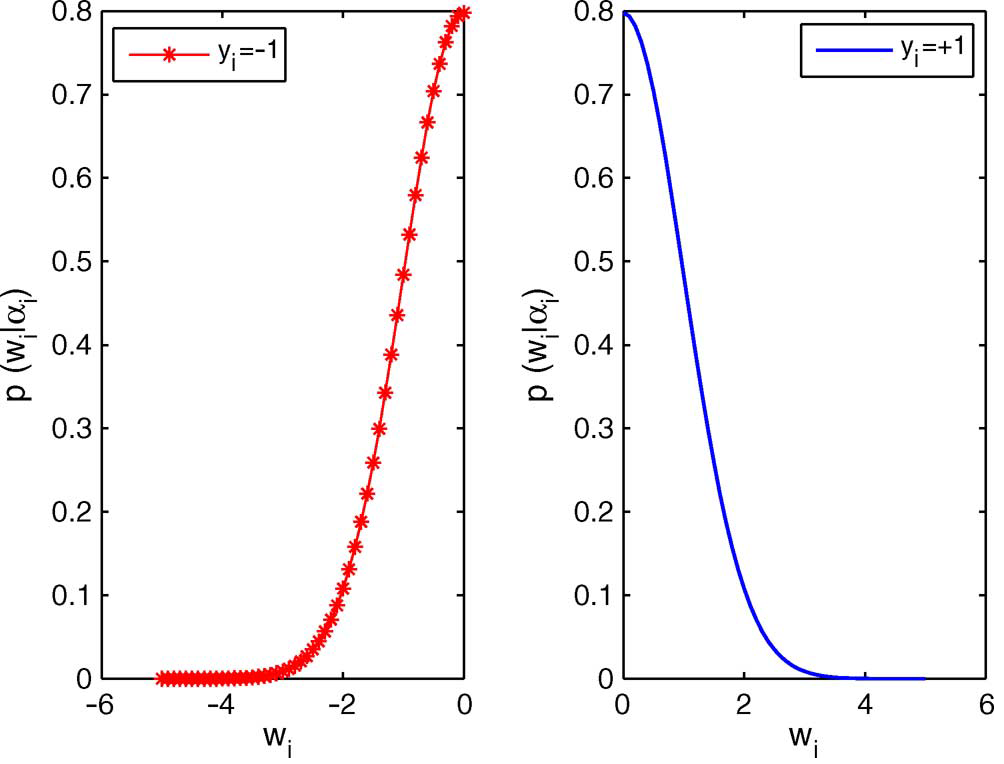
\includegraphics[width=\linewidth]{figures/TuncatedGaussian.png}\label{FigTruncGaus}}
\end{figure}
\subsection{Expectation Maximization Algorithm}\label{PcSecEM}
The \acs{PCVM} uses a simple latent variable model within the \acs{EM} algorithm.\cite{Chen.2009}
A latent variable can either be missing data or is unobservable.\cite[p. 276-277]{TrevorHastie.2009}
The latter is sometimes called hidden and can be for example class labels or parameters and has to be determined.\cite[p. 84]{Bishop.2009}
Hidden in this context means this variable can not be directly observed and his existence is implicit.\cite{Borsboom.}\\
The difference between a parameter and a latent variable in this thesis is that the parameter should be learned through the learning algorithm based on the data.
The latent variable is a part of the data which is not available (hidden) but is involved in the model.
Therefore the algorithm takes assumptions to deal with the uncertainty of this latent variables.\\
The standard probabilistic assumption is that the formulation in \eqref{EqRVMPred} is affected.
Therefore \eqref{EqRVMPred} can be reformulated as \eqref{EqPcvmRessNoise}.\cite{Chen.2009}
\begin{equation}\label{EqPcvmRessNoise}
	h_\theta (\mathbf{x}) = \boldsymbol{\Phi}_\theta(\mathbf{x}) \mathbf{w} + b +  \epsilon
\end{equation} 
With the $\theta$ parameter for the basis function and the bias $b$ instead of $w_0$.
The noise is distributed according to the standard Gaussian as $\epsilon \sim N(0,1)$.
Furthermore, because $\epsilon$ is unobservable thus latent, the $h_\theta(\mathbf{x})$ itself will be considered as latent variable.\cite{Chen.2009}\\
The \acs{PCVM} uses the probit link function, which is used for regression.\cite{Albert.1993}. It gives a variable $l = 1$, when the corresponding $h_\theta (\mathbf{x}) \ge 0$ and $l = 0$ for $h_\theta (\mathbf{x}) < 0$.\cite{Chen.2009}.
Therefore, to obtain the probit mode, the Gaussian \acs{CDF} is used.
\begin{equation}\label{EqProbitLinkProb}
	P(l=1\vert x,w,b) = p(\boldsymbol{\Phi}_\theta(\mathbf{x})\mathbf{w} + b + \epsilon \ge 0) = \Psi(\boldsymbol{\Phi}_\theta(\mathbf{x})\mathbf{w} +b)
\end{equation}
It states, given the data $\mathbf{x}$ and the parameter $\mathbf{w}$ and $b$, how likely is it that it belongs to the positive class.
To get the probability for the other class it is simply $P(l=0 \vert x,w,b) = 1-P(l=1\vert x,w,b)$.\cite{Chen.2009}\\
Revisiting \eqref{EqRVMPred}, we need to determine $\mathbf{w}$ for the model.
Again the Bayesian theorem is used to determine most probably parameter values.\cite{Chen.2009}\\
The prior for $\mathbf{w}$ is already obtain through \ref{EqPcvmNtPrior} and the bias is specified with \eqref{EqPcvmBPrior} as zero-mean Gaussian. Therefore only the likelihood has to be specified.
Taking the assumption that $h_\theta (\mathbf{x})$ is known, the Gaussian likelihood could be obtained with:\cite{Chen.2009}
\begin{equation}\label{EqPcGausLike}
\begin{gathered}
	p(\mathbf{H}_\theta(\mathbf{x})\vert w,b) = N(\mathbf{H}_\theta(\mathbf{x})\vert \mathbf{\Phi}_\theta(x)\mathbf{w}+b,1)\\
	= (2\pi)^{N/2}\exp\{-\frac{1}{2} \abs{\mathbf{H}_{\theta} - \mathbf{\Phi}_{\theta}\mathbf{w}+b\mathbf{I}}^2 \}
\end{gathered}
\end{equation}
With $\mathbf{H}_\theta(\mathbf{x}) = (h_\theta(\mathbf{x}_1),\dots,h_\theta(\mathbf{x}_N))^T$ and where $\mathbf{\Phi_\theta} = (\mathbf{\Phi}_\theta(\mathbf{x}_1)^T,\dots,\Phi_\theta(\mathbf{x}_N)^T)^T$ and $\mathbf{\Phi}_\theta(\mathbf{x_i}) = (\phi(\mathbf{x}_1,\mathbf{x}_i),\dots,(\phi(\mathbf{x}_N,\mathbf{x}_i))$ forming the kernel.
At this point it is important reintroduce a clear notation.
$\mathbf{\Phi}_\theta$ as kernel. Within this kernel $\mathbf{\Phi}(\mathbf{x}_i)$ is a row and $\mathbf{\Phi}_\theta(\mathbf{x})$ refers to the row corresponding to $\mathbf{x}$.\\
For the complete log-posterior of the parameters $\mathbf{w}$ and $b$ the corresponding parameters, $\alpha$ and $\beta$ are also considered as latent variables.
With that, there are three latent variables in the posterior.
Instead of the standard posterior, the $\log$ posterior is used and therefore has the form:\cite{Chen.2009}
\begin{equation}\label{EqPcvmInf}
\begin{gathered}
	\log p(\mathbf{w},b\vert \mathbf{y},\mathbf{H}_\theta,\alpha,\beta) \propto \log p(\mathbf{H}_\theta \vert \mathbf{w},b) + \log p(\mathbf{w}\vert \alpha) + \log p(b\vert \beta)\\
	\propto \mathbf{w}^T\mathbf{\Phi}_\theta^T(2\mathbf{H}_\theta - \mathbf{\Phi}\mathbf{w})+2b\mathbf{I}^T\mathbf{H}_\theta - 2b\mathbf{I}^T\mathbf{\Phi}_\theta - b^2N - \mathbf{w}^T\mathbf{Aw}-\beta b^2
\end{gathered}
\end{equation}
With that, we can proceed with the \acs{EM} algorithm.\cite{Chen.2009}\\
The \acs{EM} algorithm was originally introduced by Dempster et al. and is made for determining the maximum likelihood for incomplete data \cite{Dempster.1977}. 
Based on their work, many other applications are made to determine parameters.
For example Bishop used a \acs{EM} algorithm within the algorithm $k$-means cluster.\cite[p. 426-428]{Bishop.2009}
Furthermore, Hasti et al. using it in \cite[p. 272-276]{TrevorHastie.2009} for a two-component mixture model.\
Although Tipping never mentioned the use of the \acs{EM} algorithm in the \acs{RVM}, the procedure of it, explained in \ref{PcSecRVM} is similar.\cite[p. 233-234]{Tipping.2001}.
Furthermore, he introduced an Expectation-Maximisation Update approach for determining the parameters.\cite[. 235]{Tipping.2001} \newline
As the name says, it consists of two steps.
The algorithm has the $E$ and $M$ steps per iteration, and will repeat as long as a convergence criterion is reached or the maximum iteration is reached, which can be specified in algorithm \ref{PcSubSecAlgo}.
The first, the Expectation-Step finds expectations for the latent variables and furthermore an expectation for posterior of the parameters, which is referred as $\mathcal{Q}$ function.
In the case of the \acs{PCVM} it has the form:\cite{Chen.2009}
\begin{equation}\label{EqPcvmEStep}
\begin{gathered}
	\mathcal{Q}(\mathbf{w},b\vert \mathbf{w}^{old},b^{old}) = E_{\mathbf{H}_{\theta},\alpha,\beta}[\log p (\mathbf{w},b \vert \mathbf{y} ,\mathbf{H}_{\theta},\alpha,\beta) | y,\mathbf{w}^{old},b^{old}]\\
	= 2\mathbf{w}^T \mathbf{\Phi}_{\theta}^T \expB{\mathbf{H}}_\theta - \mathbf{w}^T \mathbf{\Phi}_{\theta}^T  \mathbf{\Phi}_{\theta} \mathbf{w} + 2b\mathbf{I}^T \expB{\mathbf{H}}_{\theta} -  b^2N + 2b\mathbf{I}^T \mathbf{\Phi}_\theta \mathbf{w}- \mathbf{w}^T\expB{\mathbf{A}}\mathbf{w} - \expB{\beta}b^2
\end{gathered}
\end{equation}
With $\mathbf{\expB{H}}_\theta =  E[\mathbf{H}_\theta \vert y, \mathbf{w}^{old}, b^{old}]$, $\mathbf{\expB{A}} = diag(E[\alpha_i|y_i,\mathbf{w}^{old},b^{old}])$ and $\expB{\beta}=E[\beta\vert y_i,\mathbf{w}^{old},b^{old}]$.
For details to the determination the expectation, see Appendix B in \cite{Chen.2009}.\\
This step relies on the 'old' latent variables and parameters from the previous iteration.
The next part in the iteration is the Maximization-Step.\cite{Chen.2009}\\
Revisiting \ref{EqPcvmEStep}, $\mathcal{Q}$ gives the expectation of the posterior distribution based on the current state of all variables and parameters. 
Therefore by analysing \ref{EqPcvmEStep}, the algorithm gives the most probable expectations for the posterior for the parameters with respect to the latent variables and the old parameters. \\
In this algorithm, the maximum is found by analysing the derivatives of the $\mathcal{Q}$ function with respect to $\mathbf{w}$, $b$ and $\theta$.
The latter is optimized because the Algorithm is designed to optimize his selectable parameter to avoid cross validation.\cite{Chen.2009}\\
A joint maximization of $\mathcal{Q}$ can not be done and therefore the parameters are optimized one after the other by set the derivatives to $\frac{\partial \mathcal{Q}}{\partial \mathbf{w}} = 0$ and $\frac{\partial \mathcal{Q}}{\partial b} = 0$ and solving the equation for $\mathbf{w}$ and $b$ respectively the update rules are obtained:\cite{Chen.2009}
\begin{equation}\label{EqPcvmUpdateW}
	\mathbf{w}_{new} = (\mathbf{\Phi}_\theta^T \mathbf{\Phi}_\theta + \mathbf{\expB{A}})^{-1} (\mathbf{\Phi}_\theta^T \expB{\mathbf{H}}_\theta - b\mathbf{\Phi}_\theta^T \mathbf{I})
\end{equation}
\begin{equation}\label{EqPcvmUpdateb}
	b^{new} = \frac{\mathbf{I}^T \expB{\mathbf{H}}_\theta - \mathbf{I}^T \mathbf{\Phi}_\theta \mathbf{w}}{\beta + N}
\end{equation}
With that the maximum is found and therefore the 'new' parameters for $\mathbf{w}^{old}$ and $b^{old}$ for \ref{EqPcvmEStep} are found for the next iteration.
The optimization for $\theta$ is done by a conjugate gradient algorithm\footnote{http://learning.eng.cam.ac.uk/carl/code/minimize/} which is done on basis of \eqref{EqPcvmDevTheta}.\cite{Chen.2009}
\begin{equation}\label{EqPcvmDevTheta}
	\frac{\partial \mathcal{Q}}{\partial \mathbf{\theta}_k } = 2 \sum_{i=1}^{N}\sum_{j=1}^{N} \bigg\{ (\mathbf{\Phi}_\theta \mathbf{w} - \expB{\mathbf{H}}_\theta) \mathbf{w}^T \odot (\frac{\partial\mathbf{\Phi}_\theta}{\partial \theta_k} ) \bigg\}_{(i,j)}
\end{equation}
With $\odot$ as Hadamard matrix multiplication as defined in \cite{CaroLopera.2012}.\newline
\subsection{Algorithm}\label{PcSubSecAlgo}
In the following the pseudo code of \acs{PCVM} is presented in algorithm \ref{PseudoCodePcvm}.
\begin{algorithm}[H]
	\caption{Probabilistic Classification Vector Machine}\label{PseudoCodePcvm}	
	\begin{algorithmic}[1]
		\Require $\mathbf{I}$ =\{\textbf{X,Y}\} = $\{(x_n,y_n)\}_{n=1}^{N}$ as $N$-sized training set;
		\textit{ker} as kernel type; The kernel parameter $\theta$; \textit{niter} as maximal number of iterations; \textit{threshold} as convergence criteria; \textbf{InitVector} as $N$-sized initialization vector.
		\Ensure Weight Vector $\mathbf{w}$, bias $b$ and the kernel parameter $\theta$.
		\State	[$\mathbf{w},b$] = initialize(\textbf{initVector});
		\State \textbf{nonZero} = determine\_nonZero\_Vector($\mathbf{w}$); 
		\For{$i=1$ to \textit{niter}}
			\State $\Phi$ = Calculate\_Kernel($\mathbf{X,Y}$,\textit{ker},$\theta$); 
			\State $\mathbf{w}^{new}$ = weight\_update($\mathbf{\Phi,w,Y,nonZero}$);  
			\State $b^{new}$ = bias\_update = bias\_update($\mathbf{\Phi},b,\mathbf{Y,nonZero}$);
			\State $\theta^{new}$ = parameter\_update($\mathbf{\Phi,X,Y},\mathit{ker},\theta,\mathbf{w}^{new},b^{new},\mathbf{nonZero}$);
			\State $\mathbf{nonZero}^{new}$ = determine\_nonZero\_Vector($\mathbf{w}^{new}$);
				\If{max(abs($\mathbf{w}^{new}-\mathbf{w}$)) $<$ \textit{threshold}}
					\State break;
				\Else
					\State continue;
				\EndIf
		\EndFor
	\end{algorithmic}
\end{algorithm}
\algcomment{Explanation of the Steps within the Algorithm.
	\begin{enumerate}[noitemsep]
		\item Line 1 and 2: (Random) initialization of the weight vector $\mathbf{w}$ with $N$-sized \textbf{initVector} and bias $b$. Determining non zero elements in $\mathbf{w}$ and save it as index to \textbf{nonZero}.
		\item Line 4: Calculate the kernel $\Phi$.
		\item Line 5 and 6: Update $\mathbf{w}$ and $b$ with \eqref{EqPcvmUpdateW} and \eqref{EqPcvmUpdateb} respectively.
		\item Line 7: Solve optimization problem based on \eqref{EqPcvmDevTheta}.
		\item Line 9-15: Determine the convergence by comparing the difference of $\mathbf{w}^{new}$ and $\mathbf{w}$ against the threshold. Break if convergence happens, otherwise continue.
	\end{enumerate}}\\
It can be seen in algorithm \ref{PseudoCodePcvm} that the convergence of the algorithm is only measured with the convergence behaviour of $\mathbf{w}$ and is set to $||{\mathbf{w}-\mathbf{w}^{old}}|| = 1.0e^{-3}$ in practice. 
The time complexity of the \acs{PCVM} is $\mathcal{O}(N^3)$, with N as the number of training points.\\
In practice the Cholesky decomposition is used for the matrix inversion. 
This has the computational complexity of $\mathcal{O}(M)^3$ and a memory complexity of $\mathcal{O}(M)^2$, where M is the number of non zero basis functions and is the overall complexity of the \acs{PCVM}.\cite{Chen.2009}\\
However, because of the sparsity of the prior, the \acs{PCVM} reduces the basis function from the initial start with $M = N$ to $M < N$.
In the best case it be even $M \ll N$.
An practical example of this reduction can be found in table \ref{BTableFTNev} in appendix \ref{appaB}. 
This table shows the number of vectors which are needed for the model. 
It can be seen that the \acs{PCVM} has a sparser model in comparison to the \acs{SVM} and has therefore less basis function.

\subsection{Hierachical Hyperpriors}\label{PcSubSecHierHyper}
In the section \ref{PcSecWeights} the priors are introduced with the $N$ sized parameter vector $\boldsymbol{\alpha }$ and $\beta$.
Although they are already defined, they can alternatively be controlled with hierarchical hyperparameters regarding the Bayesian Framework.
This means that hyperparameters are controlling the distribution of the prior. \cite[p. 71]{Bishop.2009}
Because these hyperparameters are controlled by a prior of another distribution, this prior is called hyperprior.\cite[.p 423]{Bishop.1995}\\
The \acs{PCVM} uses the gamma distribution for modelling the hyperprior:\cite{Chen.2009}
\begin{equation}\label{EqPcvmHyperParameter}
\begin{gathered}
		p(\boldsymbol{\alpha}) = \prod_{i=1}^{N}Gamma(\alpha_i \vert c,d)\\
		p(\beta) = Gamma(\beta\vert e,f)
\end{gathered}
\end{equation}	
With using the hyperparameters $c,d,e$ and $f$ the prior can be obtained by marginalizing out $\alpha_i$ in \ref{EqWPriorMa} and $\beta$ in \ref{EqBPriorMb}:\cite{Chen.2009}
\begin{equation}\label{EqWPriorMa}
	\begin{gathered}
		p(w_i \vert c,d) = \int_{0}^{\infty} p(w_i \vert \alpha_i)p(\alpha_i\vert ,c,d)d\alpha_i \\ 
		=\begin{dcases}
				\frac{2d^c\Gamma(c+\frac{1}{2})}{\sqrt{2\pi}\Gamma(c)}\bigg(\frac{w_i^2}{2}+d \bigg)^{-(c+\frac{1}{2})}, if y_iw_i \ge 0\\ 
				0, \>\>\>\>\>\>\>\>\>\>\>\>\>\>\>\>\>\>\>\>\>\>\>\>\>\>\>\>\>\>\>\>\>\>\>\>\>\>\>\>\>\>\>\>\>\>\>\>\>\>\>\> if y_i w_i<0
		\end{dcases}
	\end{gathered}
\end{equation}
\begin{equation}\label{EqBPriorMb}
	\begin{gathered}
		p(b\vert e,f) = \int_{0}^{\infty} p(b \vert \beta) p(\beta \vert e,f)d\beta \\
		=\frac{f^e\Gamma(e + \frac{1}{2})}{\sqrt{2\pi}\Gamma(e)}\bigg( \frac{b^2}{2}+f\bigg)^{-e+\frac{1}{2})}
	\end{gathered}
\end{equation}
Which form the hierarchical hyperprior.\cite{Chen.2014} These are equivalent to the truncated student-t prior over $\mathbf{w}$ and the student-t prior over b.\cite[p. 226]{Tipping.2001}\newline
This student-t prior is more sharply and peaked about zero than the Gaussian prior\cite{Chen.2009}, which can be seen in \cite[p. 688, 691-692]{Bishop.2009}.\newline
In practice the hyperparameters $c,d,e$ and $f$ are set to zero and therefore the prior of $\mathbf{w}$ can be formalized as in \ref{EqWPriorMwZero}.
\begin{equation}\label{EqWPriorMwZero}
	p(w_i) =
	=\begin{dcases}
	\frac{2\Gamma(\frac{1}{2})}{\sqrt{2\pi}\Gamma(0)}\bigg(\frac{w_i^2}{2} \bigg)^{-\frac{1}{2}}, if y_iw_i \ge 0\\ 
	0, \>\>\>\>\>\>\>\>\>\>\>\>\>\>\>\>\>\>\>\>\>\>\>\>\>\>\>\>\>\>\>\>\> if y_i w_i<0
	\end{dcases}
\end{equation}
The hierarchical hyperprior for $b$ can be obtained analogue to equation \eqref{EqWPriorMwZero}. This prior can be interpreted as Laplacian prior and leads to sparsity.\cite{Chen.2009} 
An idea of the multivariate Laplacian distribution can be obtained from \cite{Eltoft.2006}.
\subsection{Implementation Details}\label{PcSubSecImplementation}
In the last section of this chapter, some changes in the formulations are introduced to make the algorithm more stable in practice.
The Expectation of the latent variables for $\expB{\alpha_i}$ and $\expB{\beta}$ are calculated with:\cite{Chen.2009}
\begin{equation}\label{EqPcvmLatenHyp}
		\expB{\alpha}_i = \frac{c + \frac{1}{2}}{w_i^2 + d} \>\>\>\>\>\>\>\>\>\>\>\>\>\>\>
		\expB{\beta} = \frac{c + \frac{1}{2}}{b^2 + f}
\end{equation}
See Appendix B of \cite{Chen.2009} for details of the expectation derivation of $\expB{\alpha}_i$ and $\expB{\beta}$.\\
With that according to \ref{PcSubSecHierHyper} the hyperparameters are set to zero.
Because of the fact that $\alpha_i$ are inverse proportional to the square  $w_i$, the parameter vector can be rewritten as $\expB{A} = diag[(\sqrt{2}w_1)^{-2},\dots,(\sqrt{2}w_N)^{-2}]$.
As consequence the expectation changes to $\expB{\alpha_i} = (1/2w_i)$ and because of the sparse model many values of $w_i$ tends towards zero and therefore it may become unstable.\cite{Chen.2009}\\
Revisiting the weight may become very small and leads to large numbers in $\expB{\mathbf{A}}$. Therefore the matrix $\mathbf{M}=diag[\sqrt{2}w_1,\dots,\sqrt{2}w_N]$ with $(\mathbf{M}^{-1})^{-2}$ is used, which is suggested in \cite{Figueiredo.2003}.
This avoids the inversion of the elements $w_i$ at the update state (M-Step). This modification is applied to $b$ and $\mathbf{w}$ and therefore the equations from \ref{EqPcvmUpdateW} and \ref{EqPcvmUpdateb} changes to:\cite{Chen.2009}
\begin{equation}\label{EqPcvmStableUpdate}
	\begin{gathered}
	\mathbf{w}^{new} = \mathbf{M}(\mathbf{M \Phi}_\theta^T\mathbf{\Phi}_\theta\mathbf{M}+\mathbf{I}_n)^{-1} \mathbf{M}(\mathbf{\Phi}_\theta^T\expB{\mathbf{H}}_\theta - b \mathbf{\Phi}_\theta^T \mathbf{I}_N)\\
	b^{new} = t(1 + tNt)^{-1} t(\mathbf{I}^T\expB{H}_\theta-\mathbf{I}^T\mathbf{\Phi}_\theta\mathbf{w})
	\end{gathered}
\end{equation}
With the $N\times N$ identity matrix $\mathbf{I}$ and $t=\sqrt{2}|b|$.
Furthermore, the diagonal matrix elements of M are:
\begin{equation}\label{EqPcvmMDiag}
	m_i = \expB{\alpha_i}^{-1/2} = 
	\begin{dcases}
		\sqrt{2}w_i,\>\>\> if y_iw_i \ge 0 \\
		0, \>\>\>\>\>\>\>\>\>\>\> if y_iw_i < 0		
		\end{dcases}
\end{equation}
This changes should allow a stable numerical calculation.\\
However, this changes may not avoid the fact that some diagonal elements of $\expB{\mathbf{A}}$ in $(\mathbf{\Phi}_\theta\mathbf{\Phi}+\expB{\mathbf{A}})$ becoming very large and therefore the matrix becomes numerical singular.
This happens when $w_i$ tends towards zero.
To avoid this, the kernel column of the corresponding very small weight is deleted. \cite{Chen.2014}\newline
As already mention for the matrix inversion the Cholesky decomposition is used.\cite{Chen.2014} The Cholesky decomposition is considered as numerical stable.\cite[p. 101]{Press.2007}\\
Note that because of the zero-mean Gaussian assumption, i\,e. $N(0,1)$ the datasets for training and testing for the \acs{PCVM} has to be z-scored.
Refer to equation \eqref{EqZTrans} in section \ref{InSubSecTheta} for this.
\section{Conclusion}
Summarizing, Chen et al. have proposed the \acs{PCVM} as improvement to the \acs{SVM} and \acs{RVM}.
They have evaluated this statement, in a performance study on three synthetic datasets and 12 benchmark datasets.
They determined statistical significance with the 5x2 cv F test and the Friedman test.
The result of this study is that the \acs{PCVM} can outperform the \acs{RVM} and \acs{SVM}.
In fact the \acs{PCVM} has the same advantages over \ac{SVM} as the \acs{RVM} has and furthermore uses a more reasonable prior.\cite{Chen.2009}
